\documentclass[tikz, border=4pt]{standalone}
\usepackage{amsmath}
\usetikzlibrary{arrows.meta, decorations.pathmorphing}

% Computational domain and boundary conditions of laminar/bstep3d, not to
% scale: the channel is 12 times longer than high; the section is extruded over the width 1.5 in z. Render the PDF and the SVG
% used by the user guide next to this file with
%   pdflatex bstep3dDomain.tex && pdf2svg bstep3dDomain.pdf bstep3dDomain.svg

\begin{document}
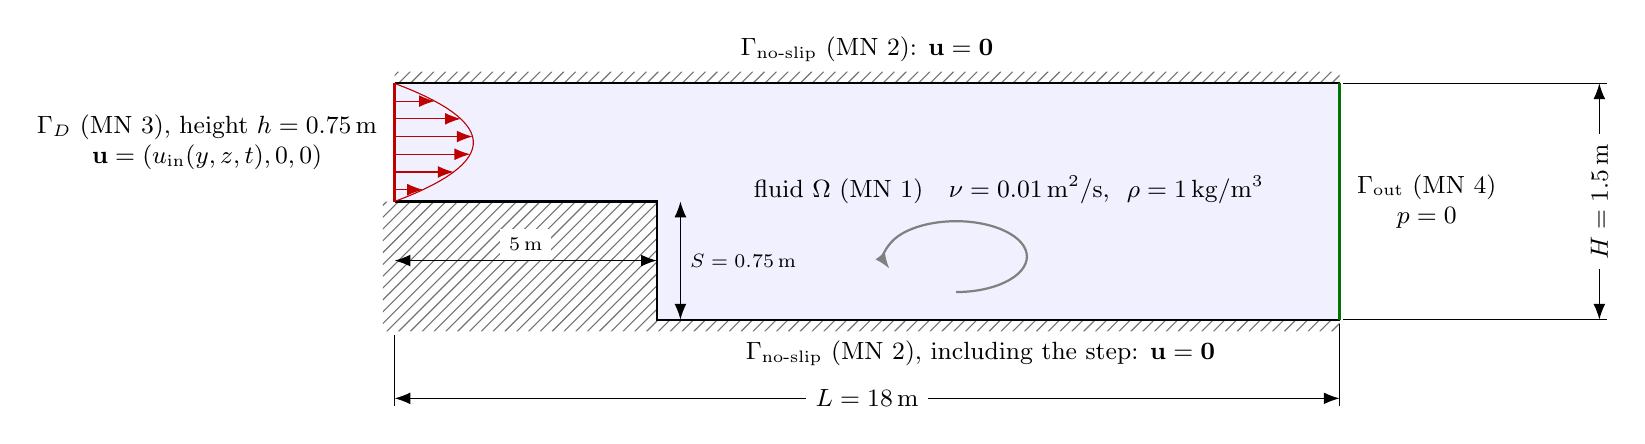
\begin{tikzpicture}[
    >={Latex[length=2mm]},
    dim/.style={<->, thin},
    label/.style={font=\small, align=center},
  ]
  \def\L{12}      % drawn length of the channel
  \def\H{3}       % drawn height of the channel
  \def\ls{3.33}   % drawn length of the step
  \def\hs{1.5}    % drawn height of the step
  \def\w{0.15}    % thickness of the hatched walls

  % fluid domain
  \fill[blue!6] (0,\hs) -- (\ls,\hs) -- (\ls,0) -- (\L,0) -- (\L,\H) -- (0,\H) -- cycle;

  % walls: top, bottom behind the step and the step itself, hatched
  \begin{scope}
    \clip (0,\H) rectangle (\L,\H+\w)
          (\ls,-\w) rectangle (\L,0)
          (-\w,-\w) rectangle (\ls,\hs);
    \foreach \x in {-4,-3.85,...,12.2}
      \draw[black!55, thin] (\x,-\w) -- ++(\H+2*\w,\H+2*\w);
  \end{scope}
  \draw[thick] (0,\H) -- (\L,\H) (0,\hs) -- (\ls,\hs) -- (\ls,0) -- (\L,0);

  % inflow: parabolic velocity profile above the step
  \draw[very thick, red!75!black] (0,\hs) -- (0,\H);
  \foreach \y in {0.1,0.25,...,0.91} {
    \pgfmathsetmacro\u{1.0*4*\y*(1-\y)}
    \draw[->, red!75!black] (0,\hs+\y*\H-\y*\hs) -- ++(\u,0);
  }
  \draw[red!75!black, thin, domain=0:1, samples=30]
    plot ({1.0*4*\x*(1-\x)}, {\hs+\x*(\H-\hs)});

  % outflow
  \draw[very thick, green!45!black] (\L,0) -- (\L,\H);

  % sketch of the recirculation behind the step
  \draw[gray, thick, ->] (\ls+3.8,0.35) arc[start angle=-90, end angle=200, x radius=0.9, y radius=0.45];

  % boundary conditions
  \node[label, left] at (-0.1,0.5*\H+0.5*\hs)
    {$\Gamma_D$ (MN 3), height $h = 0.75\,\mathrm{m}$\\ $\mathbf{u} = (u_\text{in}(y,z,t), 0, 0)$};
  \node[label, right] at (\L+0.1,0.5*\H)
    {$\Gamma_\text{out}$ (MN 4)\\ $p = 0$};
  \node[label, above] at (0.5*\L,\H+\w)
    {$\Gamma_{\mathrm{no\text{-}slip}}$ (MN 2): $\mathbf{u} = \mathbf{0}$};
  \node[label, below] at (0.62*\L,-\w)
    {$\Gamma_{\mathrm{no\text{-}slip}}$ (MN 2), including the step: $\mathbf{u} = \mathbf{0}$};

  % fluid
  \node[label] at (0.65*\L,0.55*\H)
    {fluid $\Omega$ (MN 1)\quad $\nu = 0.01\,\mathrm{m^2/s}$, \ $\rho = 1\,\mathrm{kg/m^3}$};

  % dimensions
  \draw[dim] (0,-\w-0.85) -- node[fill=white, font=\small] {$L = 18\,\mathrm{m}$} (\L,-\w-0.85);
  \draw[thin] (0,-\w-0.05) -- (0,-\w-0.95) (\L,-0.05) -- (\L,-\w-0.95);
  \draw[dim] (0,0.5*\hs) -- node[fill=blue!0, font=\scriptsize, above] {$5\,\mathrm{m}$} (\ls,0.5*\hs);
  \draw[dim] (\ls+0.3,0) -- node[font=\scriptsize, right] {$S = 0.75\,\mathrm{m}$} (\ls+0.3,\hs);
  \draw[dim] (\L+3.3,0) -- node[fill=white, font=\small, rotate=90] {$H = 1.5\,\mathrm{m}$} (\L+3.3,\H);
  \draw[thin] (\L+0.05,0) -- (\L+3.4,0) (\L+0.05,\H) -- (\L+3.4,\H);
\end{tikzpicture}
\end{document}
